% ===============================
% Data exploration
% ===============================
\newpage
\section{Accessing and exploring the Data }
\label{sec:dataaccessandexp}

As seen in the previous sections, the amount of available data in the database is enormous. In the field of computer technology, the process of scanning such a huge pool of data for potentially interesting sets is called \textit{data mining}. What is potentially interesting completely depends on the researchers intention. Therefore, a multitude of filter and visualization options should be available to facilitate the data exploration. Once a desired set of data has been identified, one should be able to export that data for further analysis. 

\subsection{Introducing miceminer}
\label{subsec:dataexp}

The \textit{miceminer} application intends to meet exactly these requirements. Basically, the application provides a user friendly interface to retrieve data from the database. Combined with some nifty filter capabilities and visualization options, the user gets a powerful tool to explore the data.

Written entirely in \textit{Flex}\footnote{Adobe Flex is a software development kit released by Adobe Systems for the development and deployment of cross-platform rich Internet applications based on the Adobe Flash platform \cite{wiki:flex}.}, the application runs within every web browser which has the $Flash^{\copyright}$ plug-in version 9 or above installed. Thus, the software is cross platform compatible, meaning that it runs on every operating system for which the $Flash^{\copyright}$ player is available. 

Furthermore, the \textit{miceminer} application doesn't need to be installed on every computer, but is stored on a computer accessible over the internet, which is called a server. Every time the application is accessed, it gets downloaded to the inquiring computer, which is called the client. This has the comfortable consequence, that each user always uses the latest version.

Additionally, \textit{Flex} offers convincing tools to build interactive user interfaces and, in conjunction with third party software, dependable ways to retrieve data from a database. Compared to \textit{Java}\footnote{Java is a programming language.[\ldots] Java application can run on any Java virtual machine (JVM) regardless of computer architecture\cite{wiki:java}.}, which has a immense \ac{API}, the \ac{API} offered by \textit{Flex} is appropriate for our needs.

More information about the \textit{miceminer} project, including screencasts which show how to use the application, \ac{API} documentation, source code and links to other resources used in the development, can be found on the project homepage at \href{http://zool-miceminer.uzh.ch/}{http://zool-miceminer.uzh.ch}\footnote{The site is only accessible from within the network of the University of Z\"urich.}. 

\subsection{Interface}
\label{subsec:miceminer_interface}

This section gives a very short introduction to the user interface. User help is found on the project homepage. Furthermore, all of the components contain a help button in the upper right corner. Clicking on this button reveals the help text for the component.

Figure \ref{fig:interface_overview} shows a screenshot of the \textit{miceminer} interface and identifies the main parts.

\begin{figure}[!ht]
\begin{center}
  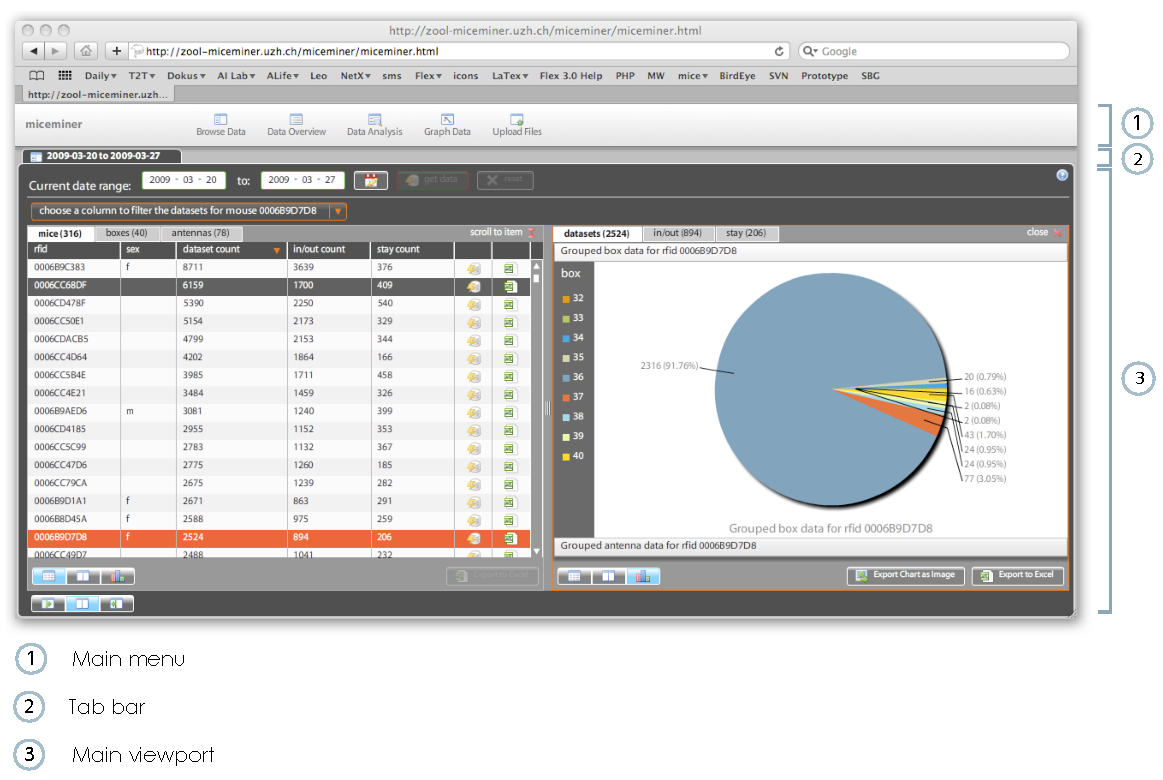
\includegraphics[width=\textwidth]{assets/pdf/interface_overview.pdf}
  \caption[miceminer interface overview]{Screenshot of the miceminer application, displaying data for a mouse and identifying the main parts of the interface.}
  \label{fig:interface_overview}
\end{center}
\end{figure}

From the \textit{main menu}, the user can start the main components listed in table \ref{tab:main_components}. 

\begin{center} 
\newcolumntype{H}{>{\bf}p{2.5cm}}
\renewcommand\arraystretch{1.5}% (MyValue=1.0 is for standard spacing)
\begin{tabularx}{\textwidth}{+>{\raggedleft\arraybackslash}H^X}

\toprule
Browse Data		& 	This is the core component of the application and contains the functionality to explore the data in the database within a definable date range. \\
Data Overview	&	Shows an overview about all the mice, boxes antennas in the database. \\
Data Analysis	&	Offers some simple data analysis and evaluation methods. \\
Graph Data		&	Interactive network representation of possible social networks within the mice community. \\
Upload Files	&	Components to perform administrative tasks. This component is password protected and is only used by the system administrators. \\\bottomrule
\end{tabularx}
\captionof{table}[miceminer main menu]{Main components selectable from the main menu within the \textit{miceminer} application.}
\label{tab:main_components}
\end{center}

If a main component is started, its interface will be shown in the main viewport, and a tab is added to the tab bar. The user can switch between the main components by clicking on the appropriate tab.

The interface arrangement is the same in all components except for the \textbf{Graph Data} component. Figure \ref{fig:interface_component} identifies the different parts with a screenshot of the \textbf{Browse Data} component.

In the parameters section, the user sets the factors influencing the data displayed in the viewport. When the help button is clicked, a window will pop up, containing instructions to use the actual component. An export to \textit{Excel} option is available in every component. Some components offer additional export formats, depending on their function. View options are only available in the \textbf{Browse Data} component.   

\begin{figure}[!htbp]
\begin{center}
  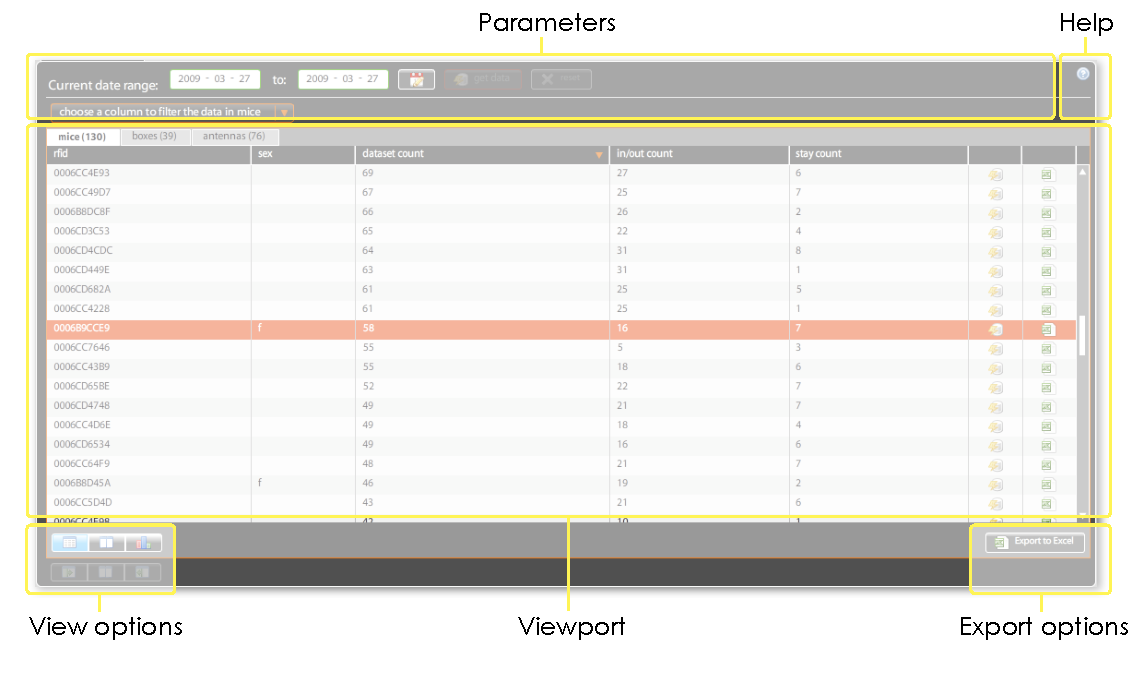
\includegraphics[width=.75\textwidth]{assets/pdf/interface_component.pdf}
  \caption[Browse Data component interface]{Screenshot of the \textbf{Browse Data} component, with labeled parts of the interface.}
  \label{fig:interface_component}
\end{center}
\end{figure}

\subsection{Software design}
\label{subsec:miceminer_design}   

\textit{Flex} itself does not include methods to query a database. Instead the application sends it's request to a \textit{PHP}\footnote{PHP is a scripting language originally designed for producing dynamic web pages\cite{wiki:php}.} file stored on the server, providing the necessary methods. These methods handle the database queries and send the results back to the \textit{Flex} application, which is running on the client computer. An auxiliary software (\textit{amfphp}\footnote{See \href{http://www.amfphp.org}{http://www.amfphp.org} for details.}) speeds up the data transfer between the server and the client.

\textit{PHP} offers convincing ways to export the data to different file formats, from which the most prominent is \textit{Excel}. A few components offer other export options, which have been designed to ensure the usage of the data in specialised data analysis software used by the researchers.

The interactions of the different software parts is illustrated in figure \ref{fig:app_design_miceminer}. Readers who are interested in the actual programming are reffered to the \textit{Additional Sites}\footnote{\href{http://zool-miceminer.uzh.ch/\#additional_sites}{http://zool-miceminer.uzh.ch/\#additional\_sites}} section on the project homepage.   

\begin{figure}[htpb]
\begin{center}
  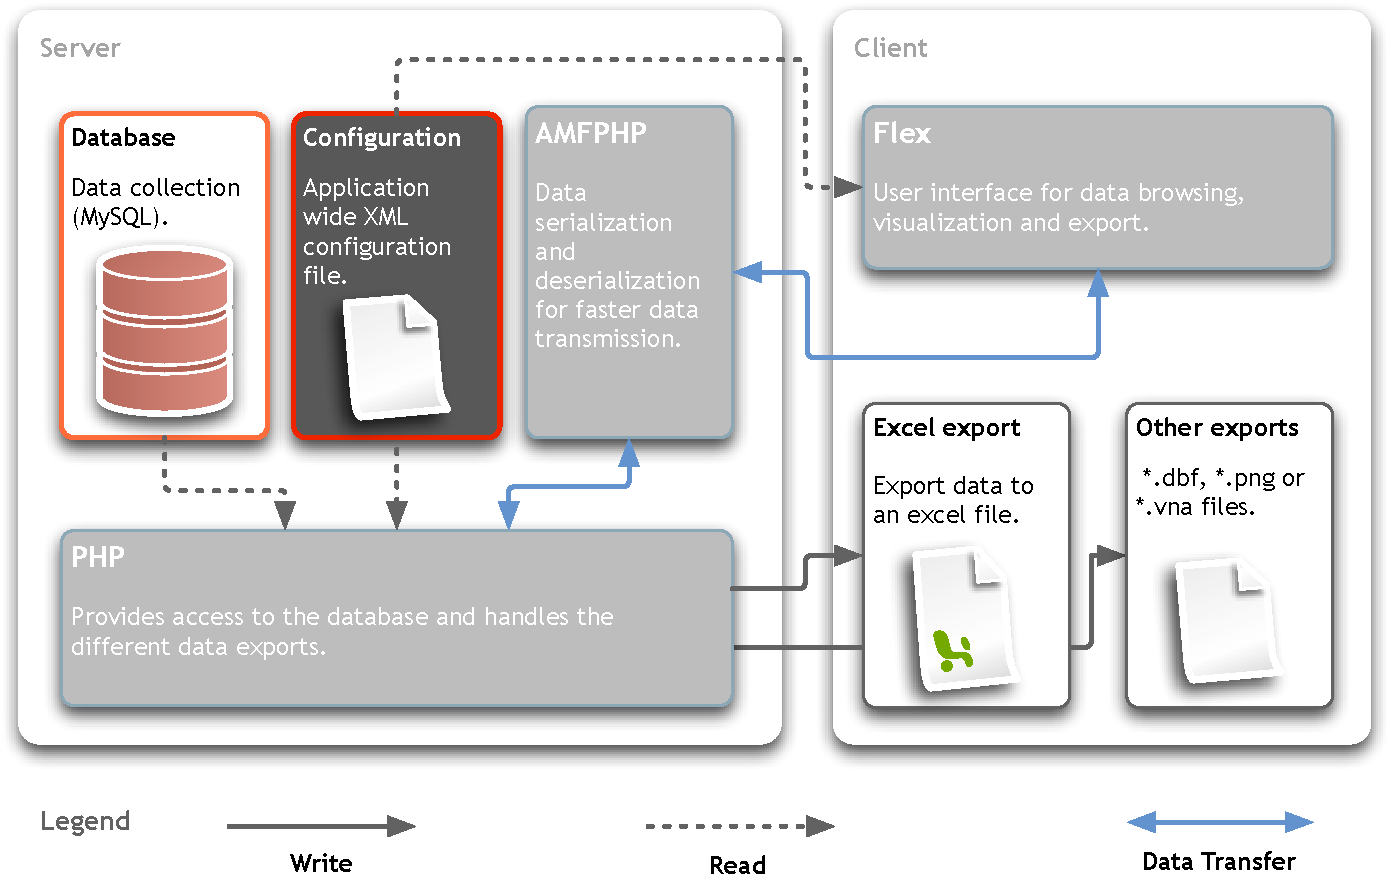
\includegraphics[width=\textwidth]{assets/pdf/application_design_miceminer.pdf}
  \caption[User interface overview]{Overview of the parts involved in the user interface.}
  \label{fig:app_design_miceminer}
\end{center}
\end{figure}

\subsection{Configuration}
\label{subsec:miceminer_config}

As pictured in Figure \ref{fig:app_design_miceminer}, the relevant parts reads its configuration from the same XML file as the data processing scripts. 

A detailed explanation of the \lstinline|<flex>| part of the configuration file, where the user interface can be configured, is beyond the scope of this document. The influence of the different values is explained on spot in the file. The clipping of the main components configuration which is shown in the appendix \ref{lst:comp_config} on page \pageref{lst:comp_config}, for instance, shows the actual configuration and the associated explanations.

The \textit{PHP} file reads the database configuration (see appendix \ref{app:configdb}) and extracts some of the values in the in the \lstinline|<flex>| configuration part as well.

The most important parameter, which can be changed easily, is the \lstinline|<maxStay>| value. This value sets the upper limit of a \textit{stay} or a \textit{meeting result} in hours, to be included in the displayed data. It had to be introduced due to the impractical duration of stay values in the \textit{stay results} (see section \ref{subsec:stayres} and \ref{subsec:meetingres} for details).   

\subsection{Basic application concept and implementation}
\label{subsec:app_concept}

On one hand, the software should offer a variety of ways and means to browse the data. On the other hand, the ease uf use should be assured. Additionaly, the technology sets its boundaries. Taking these aspects into account, as weill as the needs of the researchers and the feedbacks, the concept has been finalized during the development of the application. 

This concept is elucidated in the following sections, on the basis of the three main functionalities that the application provide. 
   
\subsubsection{Data filtering}
\label{sububsec:datafilter}

The database includes several different types of data (antenna readings, \textit{direction results}, \textit{stay results} and \textit{meeting results}) which can be allocated to the different system members (mice, boxes and antennas). Resultant are a multitude of different approaches to explore the data. One researcher, for instance, could be interested in the antenna readings of a mouse at an antenna, another one needs to know in which boxes a specific mouse has spent time. What both of these approaches share, is that the data is usually analyzed for a specific period. Hence, the selection of the period has been defined to be the starting point for every session (see figure \ref{fig:date_period}).

\begin{figure}[htpb]
\begin{center}
  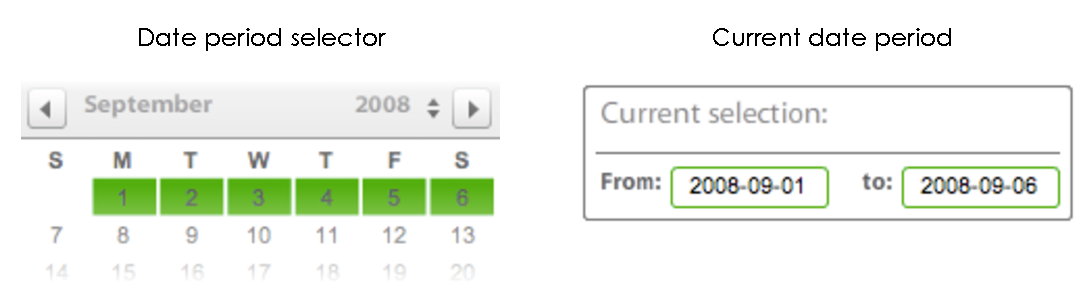
\includegraphics[width=.75\textwidth]{assets/pdf/date_period.pdf}
  \caption[Date period selection]{Date period selector and current selection.}
  \label{fig:date_period}
\end{center}
\end{figure}

The user is then provided with three tables, one with the mice, another one with the boxes, and the third one with the antennas, for which data in the selected period could be found. For each of this table elements, the exact counts of antenna recordings, \textit{direction results}, \textit{stay results} and some additional information about the item is displayed alongside (see figure \ref{fig:data_overview_with_count}). These lists aim to be a basis for the selection of interesting items. In addition, if somebody is just intersted in summarized data, he already found what he's looking for. 

\begin{figure}[htpb]
\begin{center}
  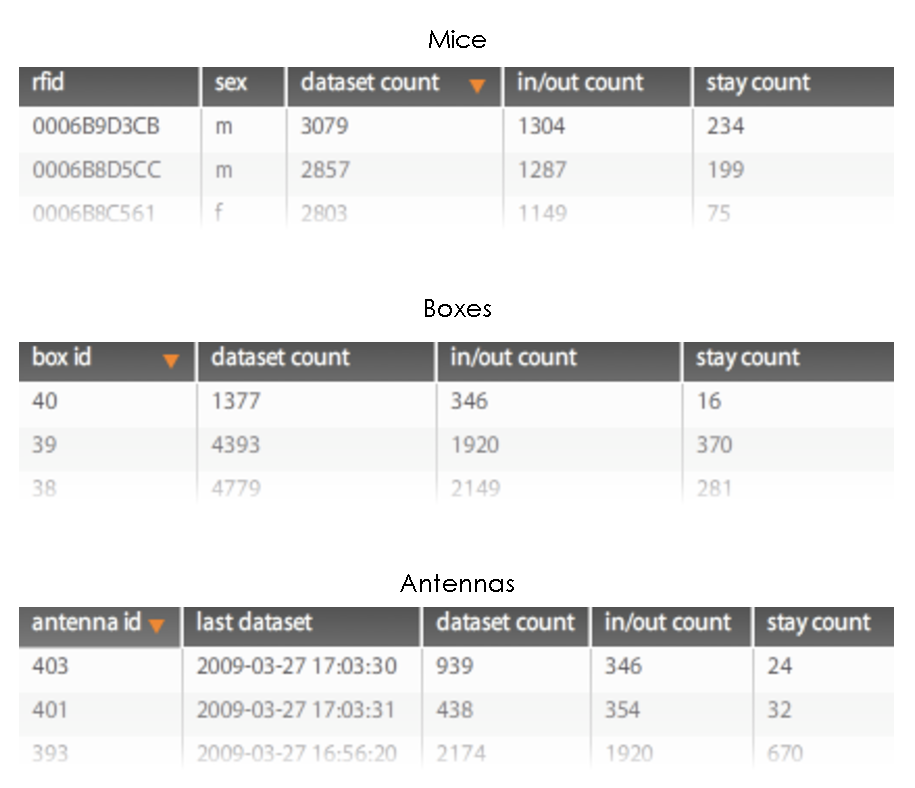
\includegraphics[width=.75\textwidth]{assets/pdf/overview_list.pdf}
  \caption[Overview of the summarized data for mice, boxes and antennas within a date period]{Overview of the mice, boxes and antennas with the respective counts for a selected period. The number of \textit{direction results} are labeled \textbf{in/out count}, the \textit{stay results}  \textbf{stay count}.}
  \label{fig:data_overview_with_count}
\end{center}
\end{figure}

With a click on the column header, the data gets sorted ascending or descending. Moreover, the data displayed in the tables can be constrained by setting filters. For each column a filter can be chosen from central a drop down menu. The menu content follows the user focus, meaning, that if the user switches to another table, the filter menu is updated to show the available column based filters for the selected table. The type of the filter depends on the kind of data the column contains. For a column containing text values, for instance, the appropriate filter is a text box where the user can type in the text to search for. Figure \ref{fig:filter_types} shows an overview of the filter types.

\begin{figure}[htpb]
\begin{center}
  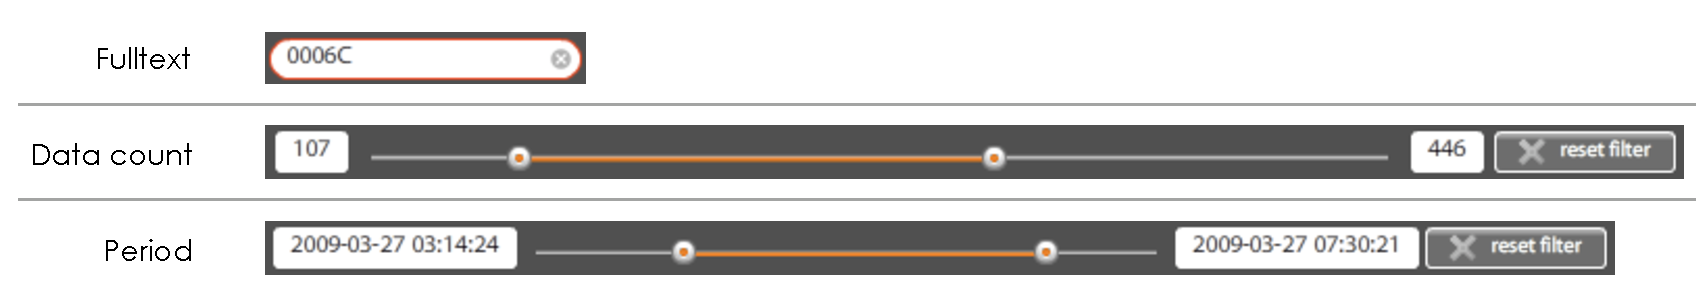
\includegraphics[width=\textwidth]{assets/pdf/filter_types.pdf}
  \caption[Filter types]{The \textit{Fulltext} filter searches the column data for the typed text. The \textit{data count} and \textit{Period} filters allow to set a lower and an upper limit by using the two sliders.}
  \label{fig:filter_types}
\end{center}
\end{figure}

Based on the tables with the summarized data, the user can choose the mice, box or antenna to get the detailed data for. Two data retrieval options are available - the first one to display the data in the \textit{miceminer} application, the second one to export data directly as an \textit{Excel} worksheet (see figure \ref{fig:get_data_options}). The latter option has been added as it allows the user to quickly download the data and analyze it in another tool. Secondly, the \textit{miceminer} application fails to display more than approximately 20,000 rows of data. With the direct \textit{Excel} export, this limit can be overcome.   

\begin{figure}[htpb]
\begin{center}
  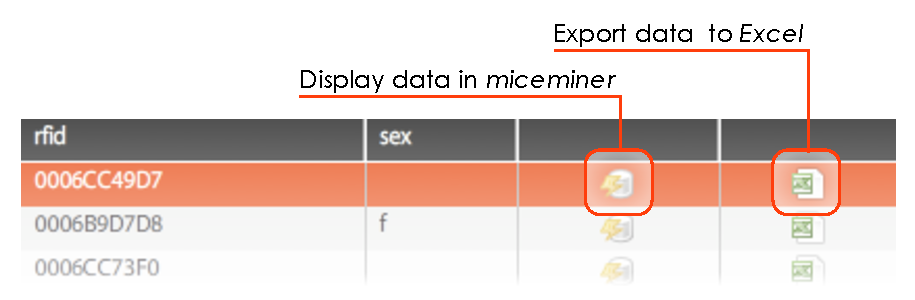
\includegraphics[width=.75\textwidth]{assets/pdf/get_data_options.pdf}
  \caption{Data retrieval options}
  \label{fig:get_data_options}
\end{center}
\end{figure}

Once the data has been load loaded into the miceminer, a secondary group of tables containing the antenna recordings, \textit{direction results} and \textit{stay results} is shown in the right part of the viewport (see figure \ref{fig:overview_data} for clippings of the tables containing the data for a mouse). The menu with the column based filters, as well as the filter mechanism is exactly the same as in the tables with the summarized data, to ensure usabilty and avoid cluttering of the interface. 

\begin{figure}[htpb]
\begin{center}
  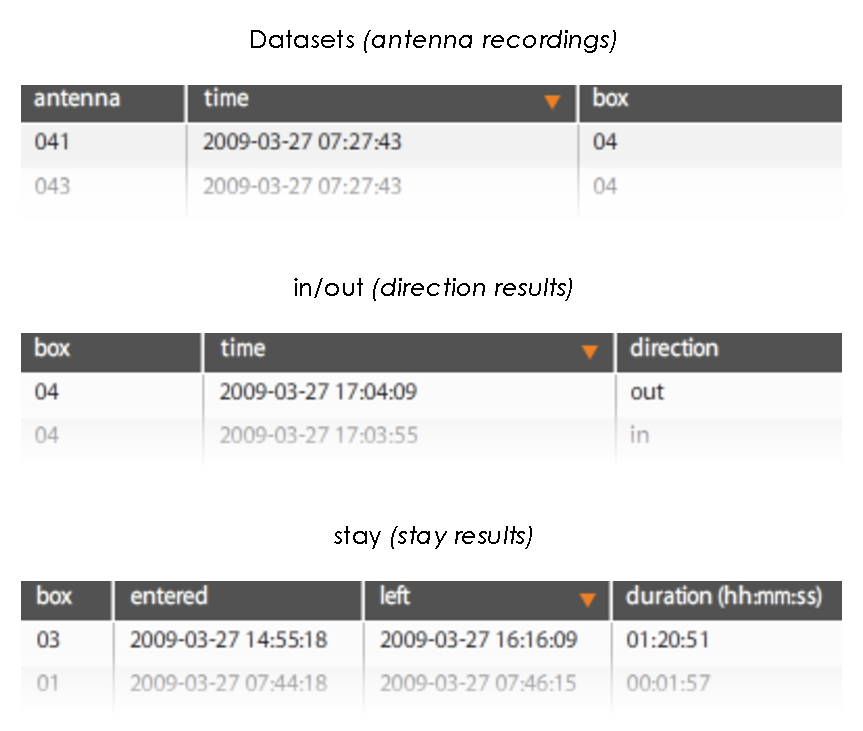
\includegraphics[width=.75\textwidth]{assets/pdf/overview_data.pdf}
  \caption{Clippings of the tables containing the antenna recordings, \textit{direction results} and \textit{stay results} for a mouse.}
  \label{fig:overview_data}
\end{center}
\end{figure}  

With the whole package of filter options, starting with the period and ending with the column filter option, the user is able to explore and export the data at every level. If the application itself is not able to handle the amount of data requested by the user, it can be exported to an \textit{Excel} sheet where the desired filters can be applied.       

\subsubsection{Data visualization}
\label{subsubsec:datavis}

Sometimes it might not be convenient to look at tables to get an idea of how an item, a mouse for instance, is positioned by its numbers in comparison to the others. Furthermore, distributions are better illustrated by the use of a pie chart. 

For the visualization of the tables containing the summarized data, the chart view displays a column chart. The x-axis values are either the mice, the boxes or the antennas with their respective counts of the antenna recordings (data count), \textit{direction results} (in/out count) and \textit{stay results} (stay count) as the y-axis values (see figure \ref{fig:mouse_chart_item} for an example of a chart item for a mouse). If the chart is visible, an option to export the chart as an image is available.

\begin{figure}[htpb]
\begin{center}
  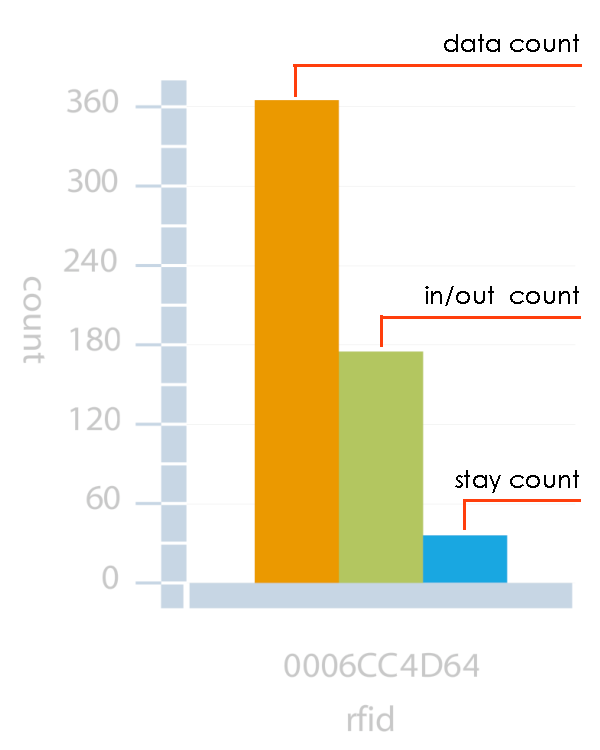
\includegraphics[width=.33\textwidth]{assets/pdf/mouse_chart_item.pdf}
  \caption[Chart item for a mouse with corresponding data counts]{Chart item for a mouse with corresponding data counts.}
  \label{fig:mouse_chart_item}
\end{center}
\end{figure}

% \begin{figure}[htpb]
% \begin{center}
%   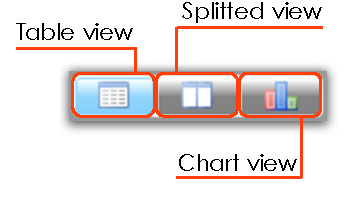
\includegraphics[width=.3\textwidth]{assets/pdf/view_options.pdf}
%   \caption[View options]{The view options for the \textbf{Browse Data} component. The splitted view is selected to get the table and the chart view side by side.}
%   \label{fig:view_options}
% \end{center}
% \end{figure}    

As in the table view, the chart view offers the same sorting, filter and export options. Furthermore, if a sort or a filter has been applied in one of the views, or another item is selected, this change is updated in the other view. This is best seen if the splitted view is selected, as shown in figure \ref{fig:table_chart_view}. Thus, the user is able to quickly find a mouse, box or antenna, which might be of special interest for further analysis.

\begin{figure}[htpb]
\begin{center}
  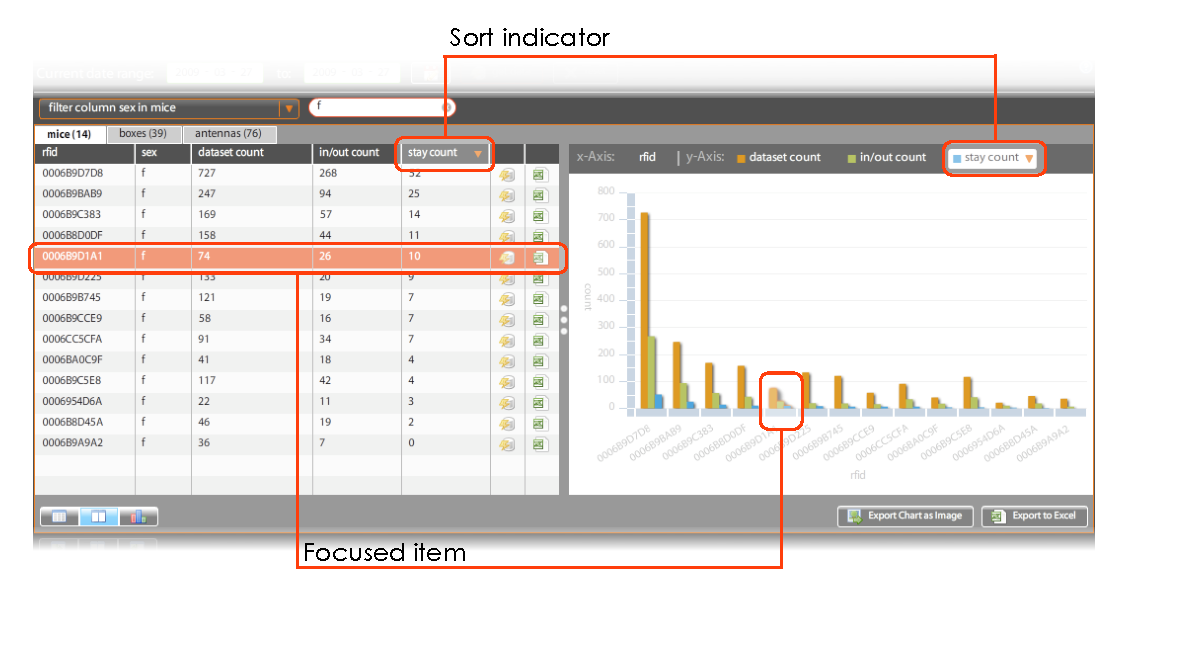
\includegraphics[width=\textwidth]{assets/pdf/table_chart_view.pdf}
  \caption[Split view]{Split view in in the \textbf{Browse Data} component. Indicated are the values which are synchronized in both, the table and the chart, views}
  \label{fig:table_chart_view}
\end{center}
\end{figure}

The chart view for the actual results of a mouse, box or antenna is different, because the reseachers are usually interested at which location a mouse has spent how many time. Therefore the data is grouped on the values in a column and displayed as a pie chart (see figure \ref{fig:pie_chart_for_mouse}). This reveals the distribution of the time spent at the different locations in a simple and clear way. 

\begin{figure}[htpb]
\begin{center}
  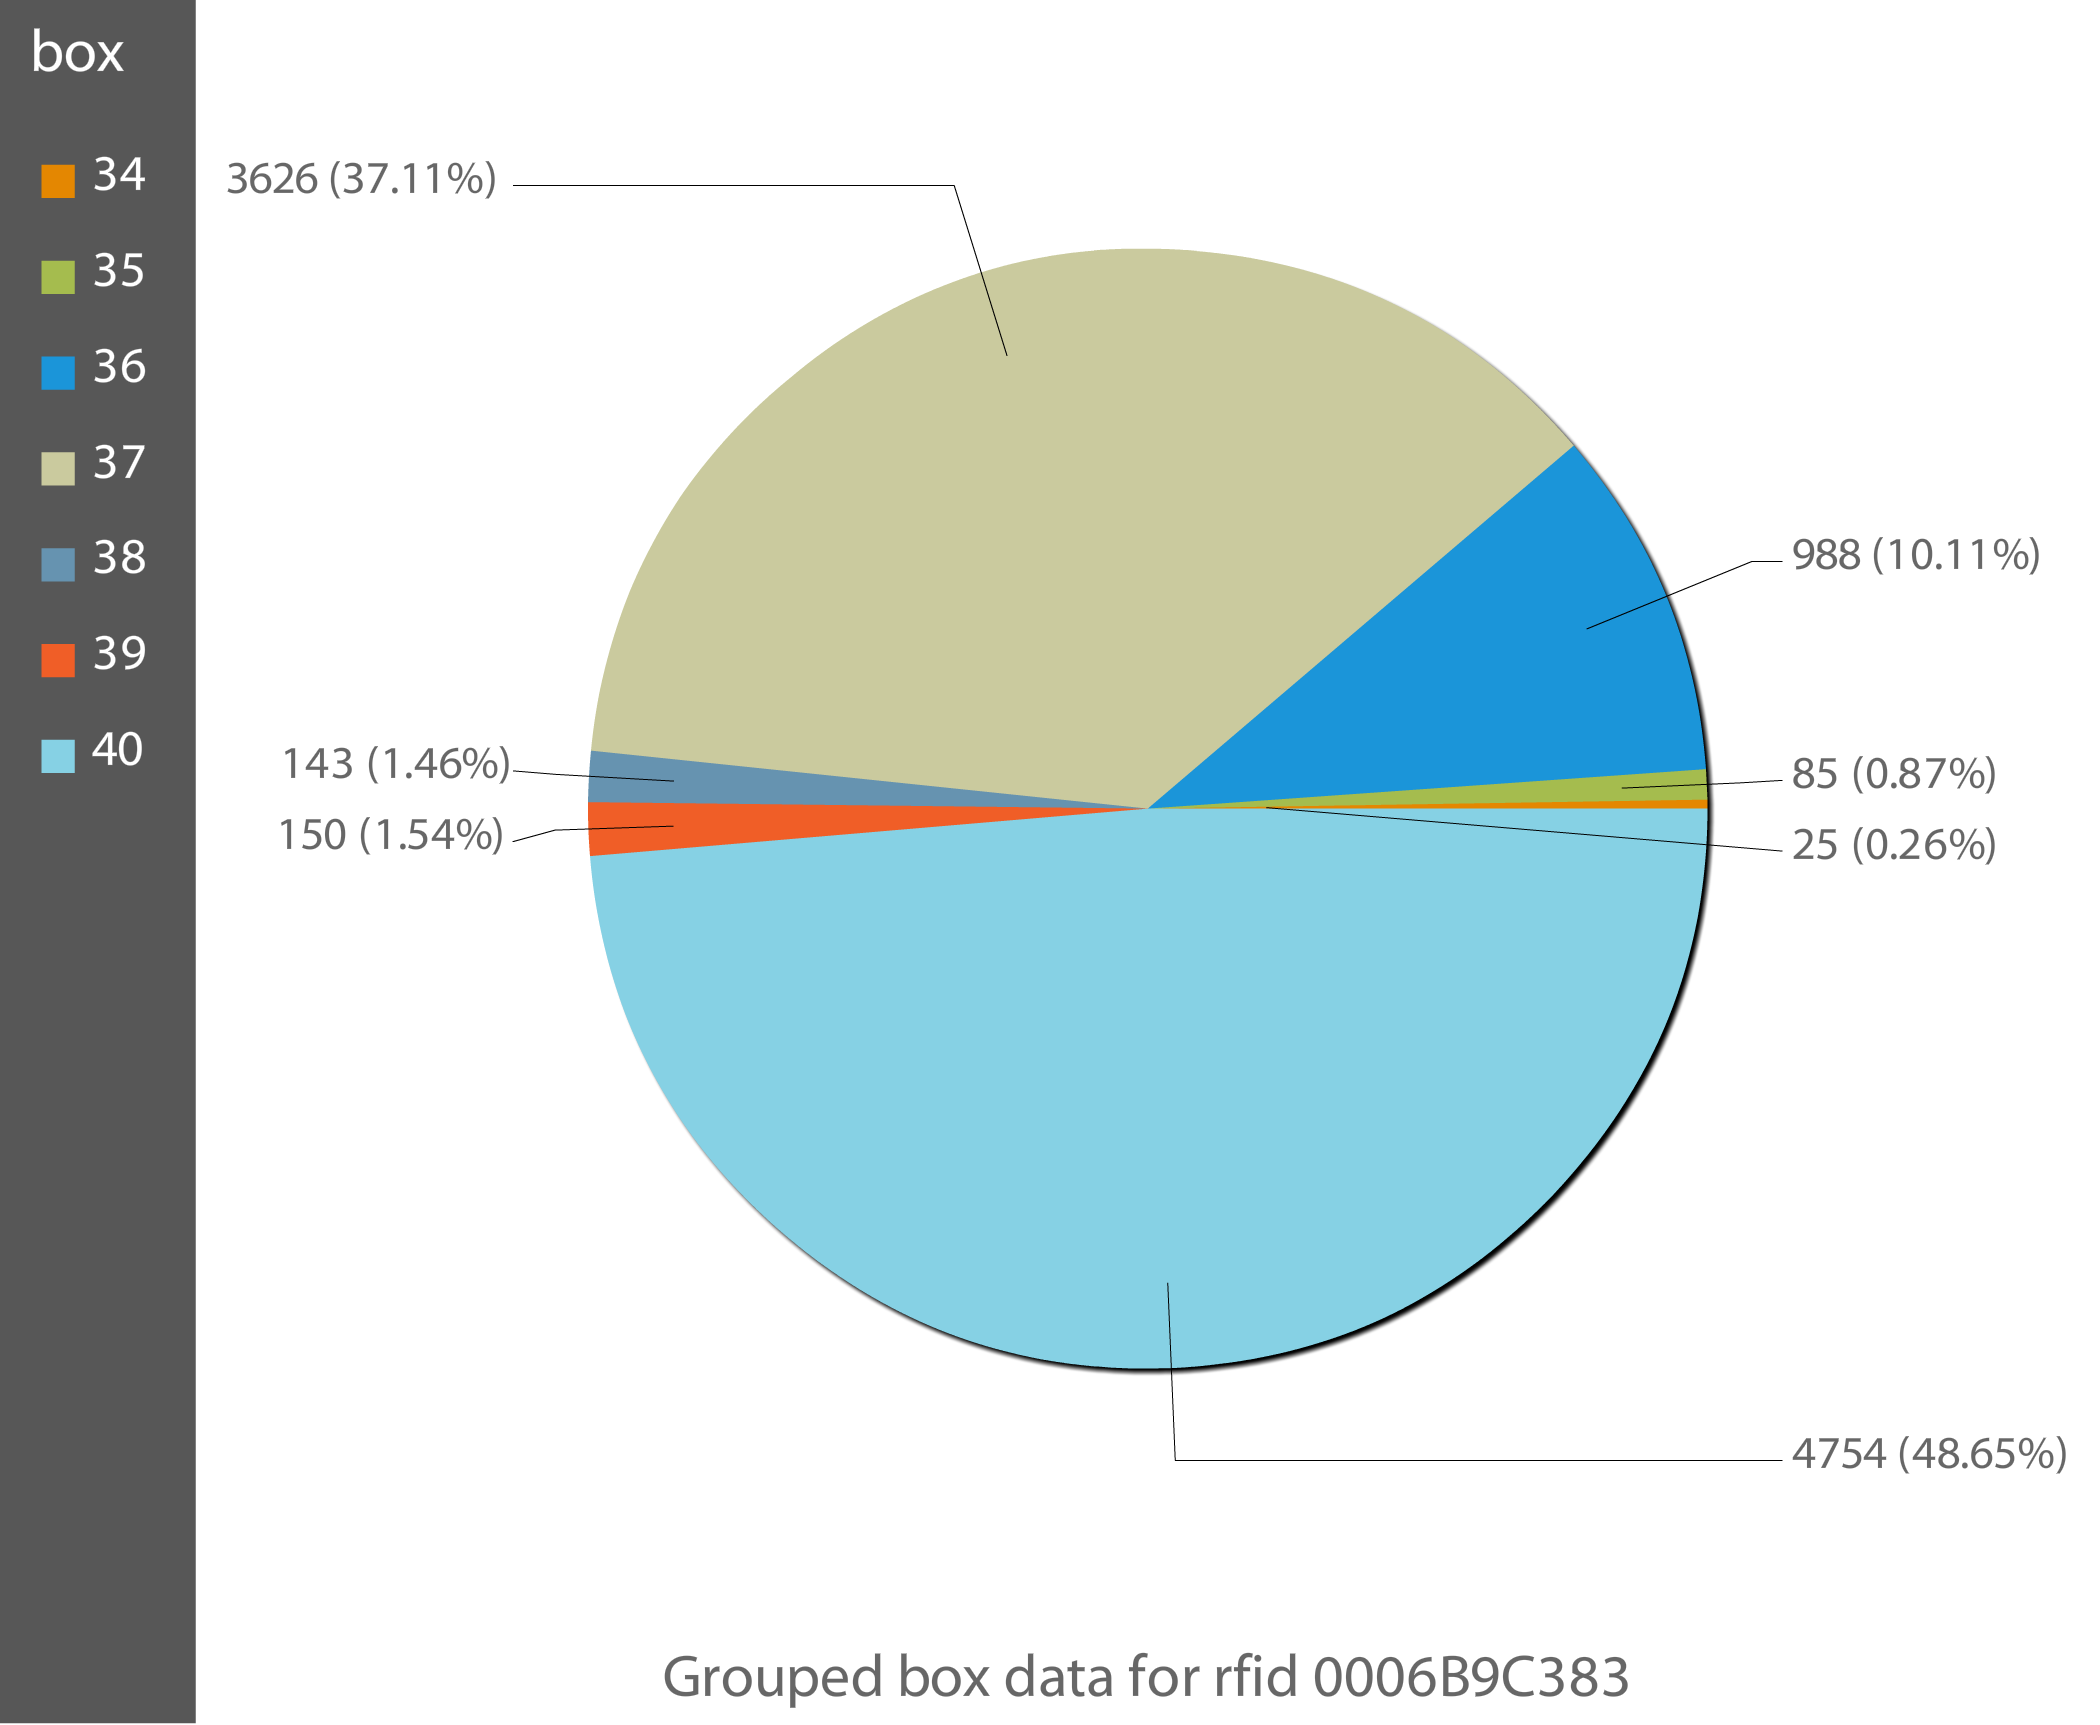
\includegraphics[width=.66\textwidth]{assets/img/pie_chart_for_mouse.png}
  \caption[Pie chart of result data for a mouse]{Pie chart with grouped box recordings for a mouse. The chart shows how many times the mouse has been recorded at the antennas of the boxes listed in the legend on the left side (e.g. 4754 times at box 40) durig the selected period.}
  \label{fig:pie_chart_for_mouse}
\end{center}
\end{figure}

When the user has selected the chart view, the \textit{Excel} export behavior changes. Not the data shown in the table will be exported, but the grouped data underlying the chart. This has been introduced according to the needs of the researchers.

In addition a secondary chart can be requested by the user. If the user double clicks a pie chart item, for example the one for box 40 as shown in figure \ref{fig:pie_chart_for_mouse}, another pie chart will be displayed alongside. In this case, the secondary chart shows which other mice have been recorded at box 40 during the period. In fact, this secondary chart is the same as if the user selects the chart view for the result of box 40 in the same period. Hence, the secondary chart is more of a handy method to view the information at the same time, side by side.

Combined with the shared filter capabilities and the export options, the visualization offers a good alternative to explore the data. A special visualization, which shows possible positive social relations between the mice living in the barn is elucidated in section \ref{sec:graph} on page \pageref{sec:graph}.

% ----------------------------------------------
% Data analysis
% ----------------------------------------------
\subsection{Simple data analysis with miceminer}
\label{subsec:data_ana} 

The \textit{miceminer} application provides some simple data analysis functionality, which have been designed based on the ideas from researchers involved in the project.

\subsubsection{Home range}
\label{subsubsec:homerangedata}

To carry out home range analysis, the positions of the nestboxes within the barn have been added to the database. The interface consists of a selector for the rfid and another one for the period the data should be retrieved for. \footnote{The data used in this component originates from the \lstinline|data| table (see section \ref{para:data_table} on page \pageref{para:data_table}).}. Once these values are set, the user can decide if the data should be exported into a file format called \textit{dBase} or if the calculation of the \textit{Minimum Convex Polygon (MCP)} should be executed. Figure \ref{fig:home_range} shows a labeled screenshot of the component interface.

\begin{figure}[htpb]
\begin{center}
  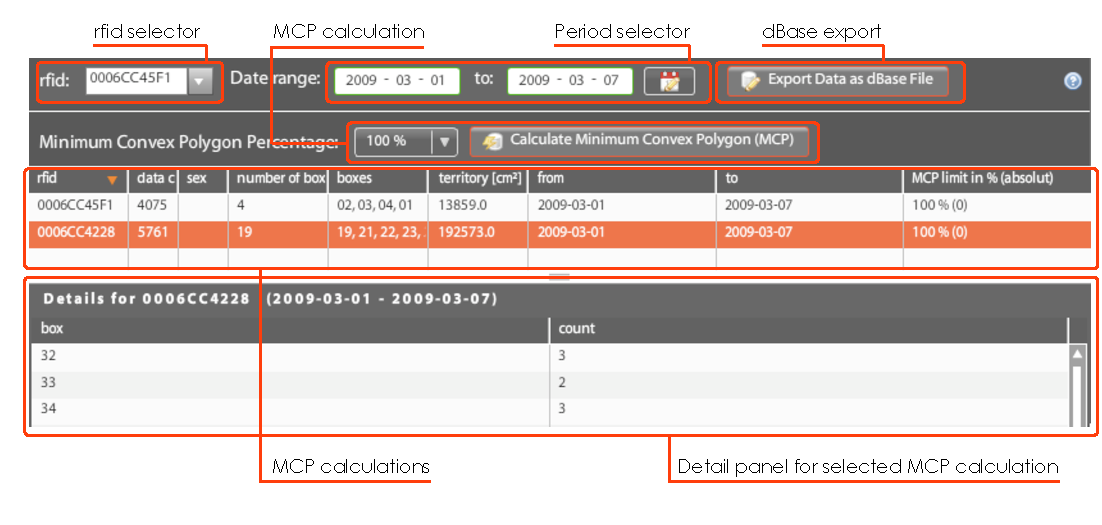
\includegraphics[width=.75\textwidth]{assets/pdf/home_range.pdf}
  \caption[Home range component interface]{Interface of the component to retrieve data for a subsequent home range analysis or MCP calculation.}
  \label{fig:home_range}
\end{center}
\end{figure}

The exported \textit{dBase} file includes all the information needed for a home range analyses using \textit{ArcGIS}\footnote{Visit \href{http://www.esri.com/software/arcgis/}{http://www.esri.com/software/arcgis/} for details about \textit{ArcGIS}.}, a software widely used for spatial analysis. 

If the selected mouse vistited more than two nestboxes in the selected period, we get a polygon spanned by the position of these nestboxes. This area can be calculated and is called the minumum convex polygon (MCP). Figure \ref{fig:mcp} shows an example for an MCP which is calculated for a mouse that visited nestboxes 12 to 17. 

\begin{figure}[htpb]
\begin{center}
  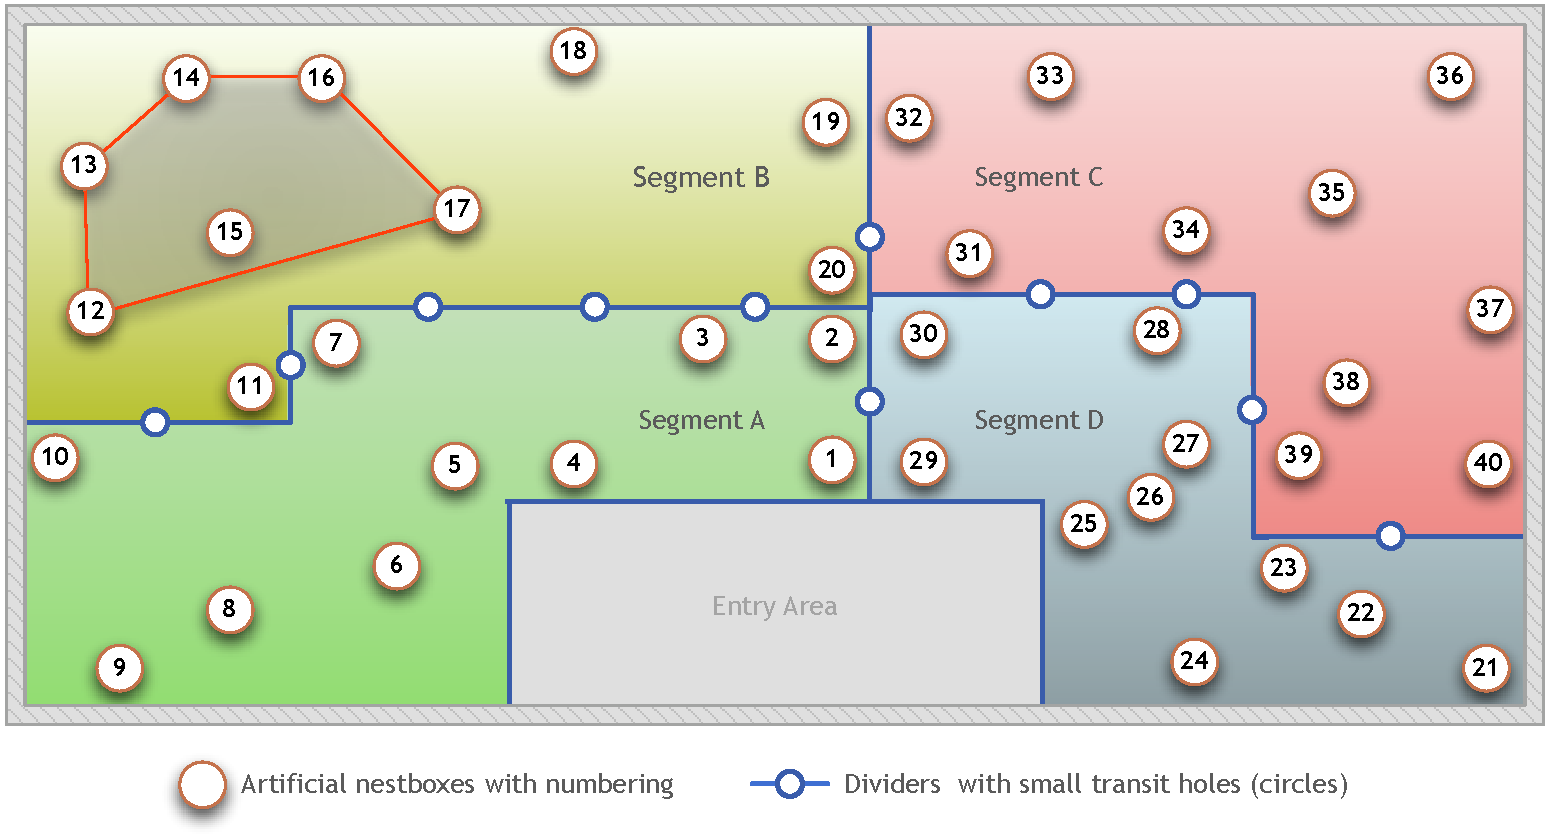
\includegraphics[width=.75\textwidth]{assets/pdf/mcp.pdf}
  \caption[Minimum convex polygon (MCP)]{An MCP for a mouse which visited nestboxes 12 to 17. In addition, the coordinate system is indicated.}
  \label{fig:mcp}
\end{center}
\end{figure}

Since this method of determining the home range is very sensible for outliers the MCP can be limited to the nestboxes with an adequate number of datasets. This is accomplished by selecting an appropriate percentage value for the MCP calculation. If the value is set 100\% percent all the nestboxes, independent of their data count, are included in the calculation. For a value of 90\%, the nestbox must have a data count which is equal or greater than 10\% of the data count for all the nestboxes. The following example which is based on the situation shown in figure \ref{fig:mcp} should clarify the method. Table \ref{tab:mcp_example} contains the distribution of the data counts for the nestboxes 12 to 17.

\begin{center} 
\newcolumntype{H}{>{}p{2cm}}
\renewcommand\arraystretch{1.2}% (MyValue=1.0 is for standard spacing)
\begin{tabularx}{.4\textwidth}{+>{\raggedright\arraybackslash}H^X}
\toprule
\rowstyle{\bfseries}
Nestbox	& 	Data count \\\midrule
12	&	44 \\
13	&	62 \\
14	&	80 \\
15	&	52 \\
16	&	12 \\
17	&	4 \\
\midrule\midrule
\rowstyle{\bfseries}
Sum	&	254
\end{tabularx}
\captionof{table}{Data count distribution for the nestboxes.}
\label{tab:mcp_example}
\end{center}

With the threshold set to 90\%, a nestbox must have at least a data count of $25.4$ (10\% of 254). Nestboxes 16 and 17 are below this value and will be excluded from the calculation. Considering figure \ref{fig:mcp}, one can see how the MCP, and therefore the home range, strikingly shrinks due to this limitation. 

The data count distribution is shown in the detail panel of the interface (labeled in figure \ref{fig:home_range}), to simplify the selection of the right percentage value.     

\subsubsection{Shared preferences}
\label{subsubsec:sharedpref}

The component is used to figure out if two female mice spent more time together in a nestbox, as expected. This is only the case if two mice have a some kind of a positive social relationship - caused by relatedness for example.

Figure \ref{fig:shared_pref} shows the component interface consisting of two controls to select the female mice and a chooser for a period. The nestbox selector allows the user to restrict the calculation to a specifc nestbox.

\begin{figure}[htpb]
\begin{center}
  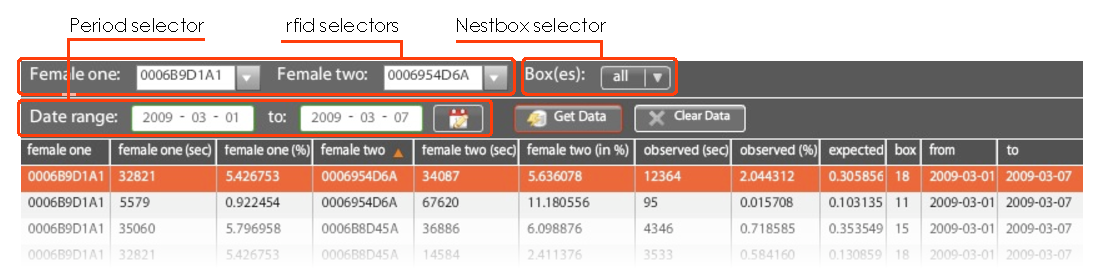
\includegraphics[width=\textwidth]{assets/pdf/shared_pref.pdf}
  \caption[Shared preference component interface]{Shared preference component interface overview.}
  \label{fig:shared_pref}
\end{center}
\end{figure}

The calculation starts by retrieving the time each of the two mice spent in a nestbox from the \lstinline|result| table (see section \ref{para:res_table} \pageref{para:res_table}). These time values are put into relation to the time the two mice spent together in a nestbox, which can be determined by querying the \lstinline|meetings| table (see section \ref{para:meetings_table} \pageref{para:meetings_table}). Resulting are a relative values for the expected and and the observed time which can be compared. 

\subsubsection{Monthly box \& Monthly antennas}
\label{subsubsec:monthbox}

Both components have been created to support Olivia Dieser in her work to determine the terretorial behavior of the mice (see \ref{subsubsec:homerange} on page \pageref{subsubsec:homerange}).

The user selects a month and optionally a period of the time of day (see figure \ref{fig:month_box_ant} for a screenshot with labeled controls) and obtains a table where the columns denote the nestboxes and each row represents a mouse. The respective data counts are found in the intersection of the nestbox column and the mouse row.

In the case of the \textbf{Monthly Box} component, the \lstinline|direction results| with a direction value of \lstinline|in| (see section \ref{para:dir_table} on page \pageref{para:dir_table}) are searched for the appropriate data. For the \textbf{Monthly Antenna} component, the data is retrieved from the \lstinline|data| table (see section \ref{para:data_table} on page \pageref{para:data_table}).

\begin{figure}[htpb]
\begin{center}
  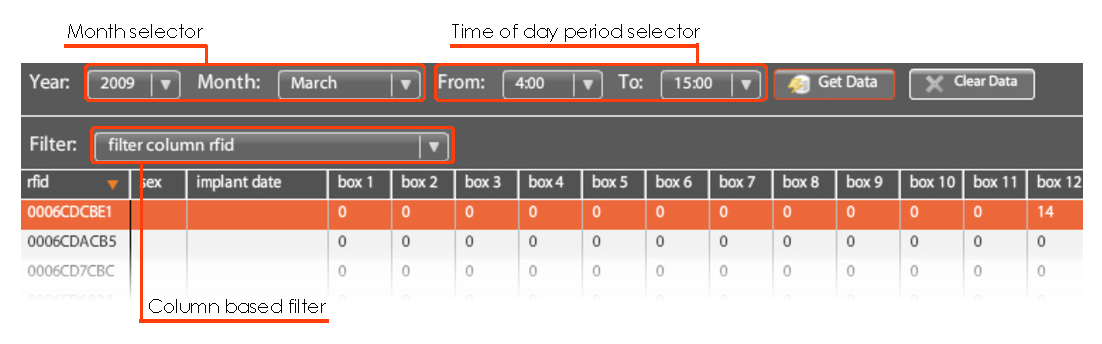
\includegraphics[width=\textwidth]{assets/pdf/month_box_ant.pdf}
  \caption[Monthly boxes component interface]{Monthly boxes component interface overview.}
  \label{fig:month_box_ant}
\end{center}
\end{figure}

The option to select a period of the time of day is used tp perform a differentiated analysis of the terretorial behavior of the mice during phases of higher and lower activity.